% ──────────────────────────────────────────────────────────────
%  Separation-Agents: LLM-Guided Multi-Agent Simulation and
%  Optimization of Rare Earth Element Separation Flowsheets
% ──────────────────────────────────────────────────────────────
\documentclass[11pt]{article}

% ── Packages ─────────────────────────────────────────────────
\usepackage[utf8]{inputenc}
\usepackage[T1]{fontenc}
\usepackage{amsmath,amssymb,amsfonts}
\usepackage{graphicx}
\usepackage{booktabs}
\usepackage{multirow}
\usepackage{hyperref}
\usepackage[margin=1in]{geometry}
\usepackage{xcolor}
\usepackage{algorithm}
\usepackage{algpseudocode}
\usepackage{caption}
\usepackage{subcaption}
\usepackage{tikz}
\usetikzlibrary{shapes.geometric,arrows.meta,positioning,fit,calc}
\usepackage{listings}
\usepackage{natbib}
\bibliographystyle{unsrtnat}

% ── Code listing style ───────────────────────────────────────
\lstset{
  basicstyle=\ttfamily\scriptsize,
  keywordstyle=\color{blue!70!black}\bfseries,
  commentstyle=\color{green!50!black}\itshape,
  stringstyle=\color{red!60!black},
  breaklines=true,
  frame=single,
  numbers=left,
  numberstyle=\tiny\color{gray},
  captionpos=b,
  language=Python,
}

% ── Metadata ─────────────────────────────────────────────────
\title{Separation-Agents: An LLM-Guided Multi-Agent Framework\\
  for Simulation and Superstructure Optimization\\
  of Rare Earth Element Separation Flowsheets}

\author{
  Step Function LLC \\
  \texttt{info@step-function.com}
}

\date{March 2026}

% ═════════════════════════════════════════════════════════════
\begin{document}
\maketitle

% ─────────────────────────────────────────────────────────────
\begin{abstract}
We present \textbf{Separation-Agents}, an open-source framework that couples
large language model (LLM) orchestration with physics-grounded simulation
and mathematical optimization for the design and analysis of rare earth
element (REE) separation flowsheets.  The framework introduces a
YAML-based domain-specific language (DSL) for declarative flowsheet
specification, two complementary simulation backends---a
sequential-modular (SM) solver backed by Reaktoro Gibbs-energy-minimization
equilibrium and a simultaneous equation-oriented (EO) solver built on
Pyomo/IPOPT---and Generalized Disjunctive Programming (GDP) for
superstructure optimization that co-selects process topology and continuous
operating parameters.  Bayesian optimization via BoTorch provides
derivative-free parameter tuning, while integrated techno-economic analysis
(TEA) and life cycle assessment (LCA) modules enable multi-criteria
screening.  All capabilities are exposed through a Model Context Protocol
(MCP) server, enabling autonomous LLM agents to propose, simulate, critique,
and optimize separation processes through natural-language interaction.  We
demonstrate the framework on two industrially relevant case studies:
(i)~equilibrium speciation and solvent extraction design for a bastn\"asite
HCl leach liquor, and (ii)~GDP-based topology optimization for REE recovery
from three unconventional waste streams (coal fly ash, acid mine drainage,
and red mud).  Results show that the GDP solver identifies optimal
topologies in $\sim$\!1.4\,s per evaluation, achieving up to 99.9\%
extraction efficiency, and that the framework's proxy OPEX and CO$_2$e
estimates are within the order-of-magnitude range of published plant data.
\end{abstract}

% ═════════════════════════════════════════════════════════════
\section{Introduction}\label{sec:intro}

The separation of rare earth elements (REEs) is among the most technically
demanding problems in industrial hydrometallurgy.  The 17~REE elements
(15~lanthanides plus yttrium and scandium) share nearly identical ionic
radii, outer-shell electronic configurations, and aqueous complex
chemistries, yielding separation factors $\beta_{A/B}$ between adjacent
lanthanides of only 1.5--3.0~\citep{xie2014critical}.  Practical separation
circuits therefore require 50--200 counter-current solvent extraction (SX)
stages per adjacent pair, with each stage requiring careful control of
extractant type, organic-to-aqueous ratio, temperature, pH, and reagent
dosage~\citep{gupta2005extractive}.

Process simulation tools for REE hydrometallurgy remain significantly less
mature than their counterparts in petroleum refining or commodity chemical
production.  Existing commercial simulators (Aspen Plus, OLI Studio, HSC
Chemistry) provide excellent thermodynamic databases but lack built-in
support for the topology-level decision making that dominates early-stage
REE circuit design---namely, the question of \emph{which} unit operations
to include and in what sequence.  Conversely, superstructure optimization
tools from the process systems engineering (PSE) community
\citep{yeomans1999systematic,grossmann2002review} offer rigorous methods
for simultaneous topology and parameter optimization via Generalized
Disjunctive Programming (GDP), but require substantial manual model
formulation effort and are difficult to use interactively.

Meanwhile, large language models (LLMs) have demonstrated remarkable
ability to interpret natural-language engineering specifications, generate
structured data, and orchestrate multi-step computational
workflows~\citep{kang2024quantitative}.  The Model Context Protocol
(MCP)~\citep{anthropic2024mcp} provides a standardized interface through
which LLM agents can invoke computational tools, receive structured
results, and iteratively refine designs---closing the loop between human
engineering intent and rigorous numerical simulation.

This paper introduces \textbf{Separation-Agents}, an open-source framework
that addresses these gaps by coupling:
\begin{enumerate}
  \item A \textbf{declarative DSL} for flowsheet specification, enabling
    LLM agents to synthesize process definitions from natural-language
    descriptions;
  \item Two \textbf{physics-grounded simulation backends}: a
    sequential-modular (SM) solver using Reaktoro~\citep{leal2015reaktoro}
    equilibrium speciation, and an equation-oriented (EO) solver using
    Pyomo/IPOPT;
  \item \textbf{GDP superstructure optimization}
    via Pyomo.GDP~\citep{chen2022pyomo} for simultaneous topology selection
    and parameter optimization;
  \item \textbf{Bayesian optimization} via BoTorch~\citep{balandat2020botorch}
    for derivative-free parameter tuning;
  \item Integrated \textbf{TEA/LCA} modules for multi-criteria screening;
  \item An \textbf{MCP server} exposing all functionality as tool endpoints
    consumable by LLM agents.
\end{enumerate}

The remainder of this paper is organized as follows.
Section~\ref{sec:background} reviews the REE separation process and
relevant computational methods.  Section~\ref{sec:architecture} describes
the framework architecture.  Section~\ref{sec:methods} details the
mathematical models.  Sections~\ref{sec:case1} and \ref{sec:case2}
present two case studies.  Section~\ref{sec:discussion} discusses
limitations and future work.  Section~\ref{sec:conclusion} concludes.


% ═════════════════════════════════════════════════════════════
\section{Background}\label{sec:background}

\subsection{REE Separation Chemistry}

REEs occur predominantly in bastn\"asite (CO$_3$F$^-$), monazite
(PO$_4^{3-}$), xenotime (PO$_4^{3-}$), and ion-adsorption clays.
Following acid or caustic leaching, the resulting liquor contains dissolved
REE ions (e.g., Nd$^{3+}$, NdCl$^{2+}$, NdCl$_2^+$, NdCl$_3$(aq),
NdCl$_4^-$) alongside gangue elements (Fe, Al, Ca, Si).  A complete
flowsheet typically comprises impurity removal, group separation, individual
REE separation via multi-stage SX, and final precipitation to oxide or
carbonate product~\citep{xie2014critical}.

The solvent extraction distribution coefficient for metal~$i$ is defined as
\begin{equation}\label{eq:D}
  D_i = \frac{[\text{M}_i]_{\text{org}}}{[\text{M}_i]_{\text{aq}}},
\end{equation}
and the separation factor between elements~$A$ and~$B$ is
$\beta_{A/B} = D_A / D_B$.  Common extractants include D2EHPA, PC88A,
Cyanex~272, and HEH[EHP], each with characteristic selectivity series
across the lanthanide row~\citep{xie2014critical}.

\subsection{Process Simulation Approaches}

Two dominant paradigms exist for chemical process simulation:
\begin{itemize}
  \item \textbf{Sequential-Modular (SM)}: Units are solved individually in
    topological order; stream states propagate forward through the
    flowsheet.  This approach is robust and natural for DAG topologies but
    does not provide analytical gradients~\citep{westerberg1979review}.
  \item \textbf{Equation-Oriented (EO)}: The entire flowsheet is
    formulated as a single system of nonlinear equations and solved
    simultaneously.  EO enables gradient-based optimization and is
    essential for superstructure formulations~\citep{biegler2010nonlinear}.
\end{itemize}

\subsection{Superstructure Optimization via GDP}

Generalized Disjunctive Programming extends mixed-integer nonlinear
programming (MINLP) by using Boolean indicator variables and disjunctions
to represent discrete topology decisions~\citep{grossmann2002review}.
A GDP formulation encodes:
\begin{itemize}
  \item \textbf{Fixed units}: always active in the flowsheet;
  \item \textbf{Optional units}: active or bypassed (binary decision);
  \item \textbf{XOR disjunctions}: exactly one of a set of alternatives
    must be active.
\end{itemize}
The GDP model is transformed to a standard MINLP via Big-M or hull
relaxation and solved by conventional NLP solvers~\citep{chen2022pyomo}.

\subsection{LLM-Guided Engineering}

Recent work has demonstrated that LLM agents, when equipped with
appropriate computational tools, can perform multi-step engineering
analyses including generating structured problem specifications,
invoking solvers, interpreting results, and proposing design
modifications~\citep{kang2024quantitative}.  The Model Context Protocol
(MCP)~\citep{anthropic2024mcp} standardizes the tool--agent interface,
enabling any MCP-compatible LLM to consume simulation capabilities without
framework-specific integration.


% ═════════════════════════════════════════════════════════════
\section{Framework Architecture}\label{sec:architecture}

Figure~\ref{fig:architecture} illustrates the Separation-Agents
architecture.  The system comprises six modules organized in a layered
design.

\begin{figure}[t]
  \centering
  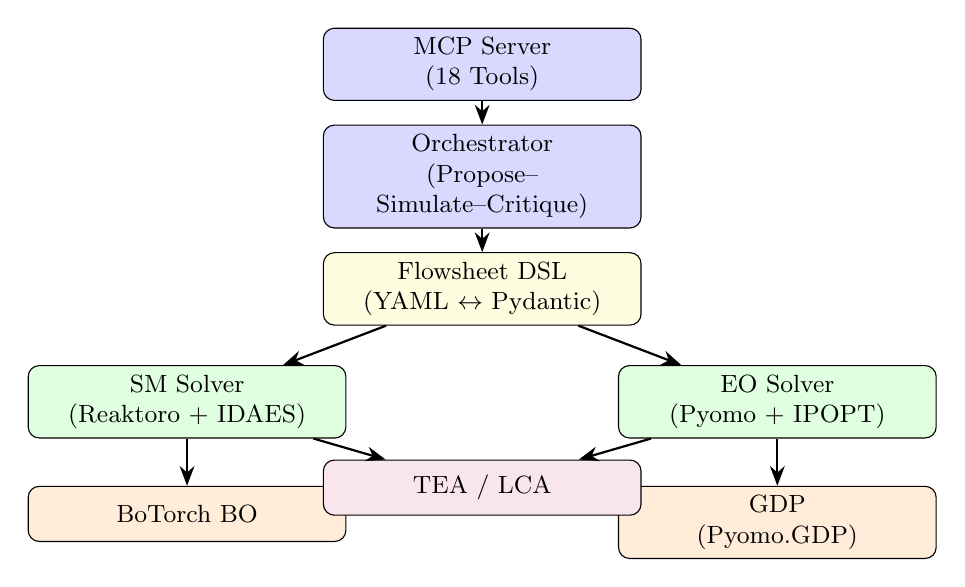
\begin{tikzpicture}[
    block/.style={rectangle, draw, rounded corners, minimum height=0.7cm,
      text width=3.8cm, align=center, font=\small},
    agent/.style={block, fill=blue!15},
    sim/.style={block, fill=green!12},
    opt/.style={block, fill=orange!15},
    cost/.style={block, fill=purple!10},
    arr/.style={-{Stealth[length=2.5mm]}, thick},
    >=Stealth,
  ]
    % Nodes
    \node[agent] (mcp)  {MCP Server\\(18 Tools)};
    \node[agent, below=0.3cm of mcp] (orch) {Orchestrator\\(Propose--Simulate--Critique)};
    \node[block, fill=yellow!12, below=0.3cm of orch] (dsl) {Flowsheet DSL\\(YAML $\leftrightarrow$ Pydantic)};
    \node[sim, below left=0.5cm and -0.3cm of dsl] (sm) {SM Solver\\(Reaktoro + IDAES)};
    \node[sim, below right=0.5cm and -0.3cm of dsl] (eo) {EO Solver\\(Pyomo + IPOPT)};
    \node[opt, below=0.6cm of sm] (bo) {BoTorch BO};
    \node[opt, below=0.6cm of eo] (gdp) {GDP\\(Pyomo.GDP)};
    \node[cost, below=1.7cm of dsl] (tea) {TEA / LCA};

    % Arrows
    \draw[arr] (mcp) -- (orch);
    \draw[arr] (orch) -- (dsl);
    \draw[arr] (dsl) -- (sm);
    \draw[arr] (dsl) -- (eo);
    \draw[arr] (sm) -- (bo);
    \draw[arr] (eo) -- (gdp);
    \draw[arr] (sm) -- (tea);
    \draw[arr] (eo) -- (tea);
  \end{tikzpicture}
  \caption{Separation-Agents architecture.  The MCP server exposes all
    simulation, optimization, and analysis capabilities as tool endpoints
    consumable by LLM agents.}
  \label{fig:architecture}
\end{figure}


\subsection{Domain-Specific Language (DSL)}

Flowsheets are defined using a Pydantic-validated DSL with three core
objects:
\begin{itemize}
  \item \textbf{Stream}: feed or intermediate stream with temperature,
    pressure, composition (weight or molar), and pH;
  \item \textbf{UnitOp}: a processing unit with a unique identifier, type,
    parameters, input streams, and output streams;
  \item \textbf{Flowsheet}: a container holding a name, a list of unit
    operations, and a list of streams.
\end{itemize}
The DSL is serializable to/from YAML, enabling LLM agents to synthesize
flowsheet definitions from natural-language descriptions and pass them
directly to the simulation backends.

\subsection{Sequential-Modular (SM) Solver}

The SM solver uses the \texttt{IDAESFlowsheetBuilder} class to:
\begin{enumerate}
  \item Topologically sort units so that each unit's inputs are produced
    by previously solved units;
  \item Propagate fully specified \texttt{StreamState} objects
    ($T, P, \mathbf{n}, \text{pH}, E_h$) through the flowsheet;
  \item Dispatch each unit to a specialized solver method backed by
    Reaktoro Gibbs-energy-minimization equilibrium.
\end{enumerate}
The SM backend is well-suited for exploratory analysis requiring rigorous
thermodynamic speciation but does not provide analytical gradients.

\subsection{Equation-Oriented (EO) Solver}

The EO solver formulates the entire flowsheet as a single Pyomo
\texttt{ConcreteModel} using a flow--composition--temperature--pressure
(FcTP) state representation.  Each unit operation is represented as a
Pyomo \texttt{Block} containing variables, constraints, and expressions.
Inter-unit connections are enforced by equality constraints linking
upstream outlet flows to downstream inlet flows.  The model is solved
simultaneously by IPOPT~\citep{wachter2006implementation}, providing
5--10$\times$ speedup over the SM backend and enabling gradient-based
optimization.

\subsection{MCP Server}

The framework exposes 18~tool endpoints through a FastMCP server,
including: \texttt{simulate\_flowsheet} (SM),
\texttt{run\_eo} (EO), \texttt{speciate\_ree\_stream},
\texttt{evaluate\_separation\_factor}, \texttt{optimize\_flowsheet}
(BoTorch), \texttt{optimize\_superstructure} (GDP), \texttt{estimate\_cost},
and \texttt{build\_ree\_flowsheet}.  Any MCP-compatible LLM agent can
invoke these tools via standard JSON-RPC, receive structured results,
and iteratively refine designs without framework-specific integration
code.


% ═════════════════════════════════════════════════════════════
\section{Mathematical Models}\label{sec:methods}

\subsection{Thermodynamic Equilibrium via Reaktoro}

All SM-backend thermodynamic calculations use
Reaktoro~\citep{leal2015reaktoro} to solve the constrained Gibbs energy
minimization:
\begin{equation}\label{eq:gibbs}
  \min_{\mathbf{n}} \; G(T, P, \mathbf{n})
    = \sum_i n_i \mu_i(T, P, \mathbf{n})
\end{equation}
subject to the elemental mass balance $\mathbf{A}\mathbf{n} = \mathbf{b}$,
where $n_i$ is the amount of species~$i$, $\mu_i$ is its chemical
potential, $\mathbf{A}$ is the formula matrix, and $\mathbf{b}$ is the
element amount vector.  The SUPCRTBL database~\citep{zimmer2016supcrtbl}
provides 300+ REE aqueous species covering all 14~stable lanthanides plus
Y and Sc, with chloride, sulfate, nitrate, fluoride, carbonate, and
hydroxide complexes.  Activity coefficients are computed via the extended
Debye-H\"uckel model (HKF equation of state).

The framework provides three pre-configured element presets:
\texttt{light\_ree} (La, Ce, Pr, Nd), \texttt{heavy\_ree} (Sm--Lu, Y, Sc),
and \texttt{full\_ree} (all 16 REE), each including appropriate base and
gangue elements.

\subsubsection{Custom Species Injection}

Many REE precipitates (hydroxides, oxalates) are absent from SUPCRTBL.
The framework dynamically injects these species using published solubility
products.  For each REE hydroxide, the standard Gibbs energy of formation
is derived from:
\begin{equation}\label{eq:ksp}
  G^0_{\text{product}} = -RT \cdot pK_{sp} \cdot \ln(10)
    + G^0_{\text{REE}^{3+}} + 3 \cdot G^0_{\text{OH}^-},
\end{equation}
using $pK_{sp}$ values from Baes and Mesmer~\citep{baes1976hydrolysis}
(e.g., $pK_{sp} = 20.7$ for La(OH)$_3$, $21.49$ for Nd(OH)$_3$).

For oxalate precipitation, a pseudo-element technique is employed to
prevent Reaktoro's Gibbs minimizer from converting oxalic acid carbon
into thermodynamically favorable inorganic species.  REE$_2$(C$_2$O$_4$)$_3$
precipitates are injected using $pK_{sp}$ values from Martell and
Smith~\citep{martell2004critical} (e.g., 25.0 for La, 28.0 for Ce,
31.14 for Nd), enabling selective fractionation by controlled oxalate
addition.


\subsection{Solvent Extraction Model}

The SX unit implements single-stage extraction:
\begin{equation}\label{eq:sx}
  \text{amt}_{\text{aq},i}
    = \frac{\text{amt}_{\text{feed},i}}{1 + D_i \cdot R_{O/A}},
\end{equation}
where $D_i$ is the distribution coefficient for species~$i$
(user-supplied or scalar) and $R_{O/A}$ is the organic-to-aqueous
volume ratio.  Aqueous background species (H$_2$O, H$^+$, OH$^-$,
Cl$^-$) have $D = 0$.

In the EO backend, $D_i$ and $R_{O/A}$ are Pyomo decision variables,
and the extraction fraction is expressed as:
\begin{equation}
  E_i = \frac{D_i \cdot R_{O/A}}{1 + D_i \cdot R_{O/A}}.
\end{equation}

\subsection{Precipitator Model}

The EO precipitator uses a recovery-fraction formulation for numerical
stability:
\begin{equation}
  \text{solid}_j = R_j \cdot \text{feed}_j,
  \qquad
  \text{barren}_j = (1 - R_j) \cdot \text{feed}_j,
\end{equation}
where $R_j \in [0, 1]$ is a decision variable.  This avoids
Ksp-based softplus formulations that cause overflow during gradient
computation.  The SM precipitator delegates to full Reaktoro equilibrium
with phase-separation logic.

\subsection{Ion Exchange Model}

The competitive Langmuir isotherm governs IX separation:
\begin{equation}\label{eq:ix}
  q_j = q_{\max} \cdot \frac{K_j \cdot c_j}{1 + \sum_k K_k \cdot c_k},
\end{equation}
where $q_{\max}$ is bed capacity, $K_j$ is the selectivity coefficient,
and $c_j$ is the feed concentration.  Recovery is capped at $\leq 1.0$
using slack decomposition (\texttt{raw\_frac = recovery + slack}) to
prevent numerical infeasibility when theoretical loading exceeds feed.


\subsection{GDP Superstructure Formulation}\label{sec:gdp}

The GDP module formulates the superstructure as:
\begin{subequations}\label{eq:gdp}
\begin{align}
  \min_{\mathbf{x}, \mathbf{Y}} \quad & f(\mathbf{x}, \mathbf{Y}) \\
  \text{s.t.} \quad
    & \bigvee_{k \in \mathcal{D}_j}
      \begin{bmatrix}
        Y_{j,k} \\ h_{j,k}(\mathbf{x}) \leq 0
      \end{bmatrix}
      \quad \forall j \in \mathcal{J} \\
    & \text{Exactly one } Y_{j,k} = \text{True}
      \quad \forall j \in \mathcal{J} \\
    & g(\mathbf{x}) \leq 0,
\end{align}
\end{subequations}
where $\mathbf{x}$ are continuous variables (flows, $D_i$, $R_{O/A}$),
$\mathbf{Y}$ are Boolean indicator variables, $\mathcal{J}$ indexes
disjunctions, and $\mathcal{D}_j$ indexes alternatives within
disjunction~$j$.

When a unit is bypassed, passthrough constraints enforce:
\begin{equation}
  \text{outlet}_j = \text{inlet}_j \quad \forall j \in \text{components},
\end{equation}
ensuring mass balance closure regardless of topology.  The GDP model is
converted to MINLP via Big-M relaxation using
\texttt{TransformationFactory('gdp.bigm')} and solved by IPOPT.


\subsection{Bayesian Optimization}

For derivative-free parameter optimization, the framework uses
BoTorch's \texttt{SingleTaskGP}---an exact Gaussian process with
Mat\'ern~5/2 kernel and automatic relevance determination---fitted
by marginal log-likelihood maximization.  The acquisition function is
Log Expected Improvement (LogEI)~\citep{ament2024logei}:
\begin{equation}
  \text{LogEI}(\mathbf{x}) = \log\!\left(
    \mathbb{E}\!\left[\max\!\left(
      f(\mathbf{x}) - f^*_{\text{best}},\; 0
    \right)\right]
  \right),
\end{equation}
which avoids the numerical instabilities of standard EI.  The BO loop
uses Latin Hypercube initialization (5 points) followed by 15 sequential
acquisitions, each optimized via multi-start L-BFGS-B with 5 restarts.


\subsection{Techno-Economic Analysis and LCA}

Proxy OPEX is computed by summing reagent costs, pumping energy, and
unit energy consumption:
\begin{equation}
  \text{OPEX} = \sum_{s} \sum_i n_i \frac{M_i}{1000} p_i
    + C_{\text{pump}} V_{\text{water}}
    + \sum_u E_u \cdot p_{\text{elec}},
\end{equation}
where $p_i$ is the reagent price (\$/kg), $C_{\text{pump}} = 0.05$~\$/m$^3$,
$E_u$ is unit energy (kWh), and $p_{\text{elec}} = 0.08$~\$/kWh.
The LCA module mirrors this structure using cradle-to-gate CO$_2$e
emission factors in place of prices (e.g., 1.10~kgCO$_2$e/kg for HCl,
1.20 for NaOH, 2.50 for HNO$_3$).

These are proxy values suitable for screening-level comparisons; for
publication-grade TEA/LCA, process-specific data from chemical market
databases and ecoinvent should be used.


% ═════════════════════════════════════════════════════════════
\section{Case Study 1: Speciation and SX Design for Bastn\"asite Leach Liquor}\label{sec:case1}

\subsection{Problem Description}

We consider an HCl leach liquor from bastn\"asite processing containing
La$^{3+}$, Ce$^{3+}$, and Nd$^{3+}$ at 10~mmol/L each in 0.5~M HCl
at 25$^\circ$C---representative of a typical primary LREE
feed~\citep{xie2014critical}.  The objective is to characterize the
aqueous speciation, design a two-unit SX--precipitator flowsheet, and
optimize the organic-to-aqueous ratio for minimum OPEX.

\subsection{Equilibrium Speciation}

Using the \texttt{speciate\_ree\_stream} MCP tool with the
\texttt{light\_ree} database preset, Reaktoro computes the equilibrium
distribution at pH~0.34.  Table~\ref{tab:speciation} summarizes the
dominant species.

\begin{table}[t]
  \centering
  \caption{Equilibrium speciation of La, Ce, and Nd in 0.5~M HCl
    at 25$^\circ$C (amounts in mmol).}
  \label{tab:speciation}
  \begin{tabular}{@{}llc@{}}
    \toprule
    Element & Species & Amount (mmol) \\
    \midrule
    \multirow{4}{*}{La}
      & La$^{3+}$       & 4.73 \\
      & LaCl$^{2+}$     & 4.24 \\
      & LaCl$_2^+$      & 0.83 \\
      & LaCl$_3$(aq)    & 0.16 \\
    \midrule
    \multirow{4}{*}{Ce}
      & Ce$^{3+}$       & 4.66 \\
      & CeCl$^{2+}$     & 4.18 \\
      & CeCl$_2^+$      & 0.97 \\
      & CeCl$_3$(aq)    & 0.16 \\
    \midrule
    \multirow{4}{*}{Nd}
      & Nd$^{3+}$       & 4.65 \\
      & NdCl$^{2+}$     & 4.17 \\
      & NdCl$_2^+$      & 0.97 \\
      & NdCl$_3$(aq)    & 0.19 \\
    \bottomrule
  \end{tabular}
\end{table}

Several observations are noteworthy.  First, the free-ion fraction
decreases across the series (La: 47.3\%, Ce: 46.6\%, Nd: 46.5\%),
consistent with increasing chloride complexation stability from La to
Nd reported by Migdisov et al.~\citep{migdisov2009experimental}.  Second,
the mono-chloride complex (REECl$^{2+}$) is the second most abundant
species for all three elements, consistent with formation constant data
in the SUPCRTBL database.  Third, the computed ionic strength of 0.54~M
indicates moderate non-ideality requiring the extended Debye-H\"uckel
activity model, which is automatically applied.

\subsection{Flowsheet Simulation}

A two-unit flowsheet (SX $\rightarrow$ Precipitator) is constructed
with distribution coefficients $D_{\text{La}} = 2.0$,
$D_{\text{Ce}} = 5.0$, and $D_{\text{Nd}} = 3.5$ (representative
of D2EHPA at moderate HCl~\citep{xie2014critical}), and
$R_{O/A} = 1.0$.  The EO solver converges in 1.8\,s and produces
the results in Table~\ref{tab:sx_results}.

\begin{table}[t]
  \centering
  \caption{SX extraction fractions and flowsheet KPIs for the
    bastn\"asite leach liquor (EO solver).}
  \label{tab:sx_results}
  \begin{tabular}{@{}lcc@{}}
    \toprule
    Metric & Value & Unit \\
    \midrule
    $E_{\text{La}}$ & 0.667 & --- \\
    $E_{\text{Ce}}$ & 0.833 & --- \\
    $E_{\text{Nd}}$ & 0.778 & --- \\
    Precipitator REE recovery & 0.963 & --- \\
    Proxy OPEX & 5.58 & USD \\
    CO$_2$e & 13.94 & kg CO$_2$e/kg REE \\
    Solve time & 1.8 & s \\
    \bottomrule
  \end{tabular}
\end{table}

The extraction fractions follow the expected selectivity order
($E_{\text{Ce}} > E_{\text{Nd}} > E_{\text{La}}$), and the OPEX per
kilogram of REE product (\$7.08/kg) falls within the order-of-magnitude
range of published estimates (\$15--60/kg REO per~\citet{golev2014rare}).
The CO$_2$ intensity of 13.94~kgCO$_2$e/kg REE is consistent with the
5--25~kgCO$_2$e/kg range reported by~\citet{zaimes2015design}.


\subsection{Benchmark Validation}

The framework's benchmark suite (11/11 tests passing) validates:
\begin{itemize}
  \item Temperature sensitivity (25--80$^\circ$C) with monotonic
    pH and free-ion fraction shifts;
  \item Mixed REE/Fe/Al speciation in chloride media (40 species);
  \item REE recovery within published plant ranges (60--95\%);
  \item Reagent consumption scaling (OPEX ratio 1.98$\times$ at
    2$\times$ feed, $<$1\% deviation per-kg-ore);
  \item OPEX and CO$_2$e within order-of-magnitude of published data;
  \item Robustness: zero-REE feed, single-unit flowsheets, extreme
    acid (5~M HCl, pH $= -0.50$).
\end{itemize}


% ═════════════════════════════════════════════════════════════
\section{Case Study 2: GDP Topology Optimization for Waste Stream REE Recovery}\label{sec:case2}

\subsection{Problem Description}

Unconventional REE sources---coal fly ash, acid mine drainage (AMD),
and red mud---represent enormous untapped reserves but pose unique
challenges: dilute concentrations (0.05--3.5~g/L REE), extreme pH
(0.8--3.5), and high gangue-to-REE ratios (up to 100:1).  The optimal
process topology depends strongly on feed characteristics, making this
an ideal application for superstructure optimization.

We evaluate six candidate topologies for each waste stream:
\begin{itemize}
  \item[\textbf{A}:] SX only (baseline);
  \item[\textbf{B}:] SX $\rightarrow$ Precipitator;
  \item[\textbf{C}:] IX $\rightarrow$ SX (pre-concentration then
    separation);
  \item[\textbf{D}:] IX $\rightarrow$ Precipitator (no SX);
  \item[\textbf{E}:] SX $\rightarrow$ Precipitator $\rightarrow$ IX
    (full chain);
  \item[\textbf{F}:] GDP auto-select (optional precipitator and IX,
    SX fixed).
\end{itemize}

\subsection{Waste Stream Definitions}

Table~\ref{tab:waste} defines the three feed streams.

\begin{table}[t]
  \centering
  \caption{Waste stream feed compositions (g/L basis, 1~kg H$_2$O).}
  \label{tab:waste}
  \begin{tabular}{@{}lcccc@{}}
    \toprule
    Stream & La$^{3+}$ & Ce$^{3+}$ & Nd$^{3+}$ & pH \\
    \midrule
    Coal fly ash  & 0.80 & 1.50 & 0.50 & 1.5 \\
    AMD           & 0.05 & 0.10 & 0.03 & 3.5 \\
    Red mud       & 2.00 & 3.50 & 1.20 & 0.8 \\
    \bottomrule
  \end{tabular}
\end{table}


\subsection{Results}

Table~\ref{tab:gdp_results} summarizes the route comparison.  All
18~evaluations (6~routes $\times$ 3~streams) solve successfully.
Routes~A--E are solved using the EO backend with
\texttt{minimize\_opex}; Route~F uses the GDP solver with
\texttt{maximize\_recovery}.

\begin{table*}[t]
  \centering
  \caption{Route comparison across three waste streams.  OPEX is proxy
    operating cost (USD); $E_{\text{Ce}}$~is cerium extraction fraction;
    Recovery is overall REE recovery; Time is wall-clock solve
    time~(s).}
  \label{tab:gdp_results}
  \begin{tabular}{@{}llcccccccc@{}}
    \toprule
    & & \multicolumn{2}{c}{Coal Fly Ash}
    & & \multicolumn{2}{c}{AMD}
    & & \multicolumn{2}{c}{Red Mud} \\
    \cmidrule{3-4} \cmidrule{6-7} \cmidrule{9-10}
    Route & Topology
      & OPEX & Recov.
      & & OPEX & Recov.
      & & OPEX & Recov. \\
    \midrule
    A & SX only
      & \$5.58 & 0.833
      & & \$5.56 & 0.833
      & & \$5.60 & 0.833 \\
    B & SX $\rightarrow$ Precip
      & \$5.58 & 0.963
      & & \$5.56 & 0.964
      & & \$5.60 & 0.963 \\
    C & IX $\rightarrow$ SX
      & \$15.58 & 0.007
      & & \$15.56 & 0.096
      & & \$15.60 & 0.003 \\
    D & IX $\rightarrow$ Precip
      & \$10.58 & 0.960
      & & \$10.56 & 0.960
      & & \$10.60 & 0.960 \\
    E & SX $\rightarrow$ Precip $\rightarrow$ IX
      & \$15.58 & 0.963
      & & \$15.56 & 0.964
      & & \$15.60 & 0.963 \\
    F & GDP auto
      & ---    & \textbf{0.999}
      & & ---    & \textbf{0.999}
      & & ---    & \textbf{0.999} \\
    \midrule
    \multicolumn{2}{l}{F solve time}
      & \multicolumn{2}{c}{1.42\,s}
      & & \multicolumn{2}{c}{1.38\,s}
      & & \multicolumn{2}{c}{1.38\,s} \\
    \bottomrule
  \end{tabular}
\end{table*}

\subsection{Analysis}

Several findings emerge from the route comparison:

\textbf{GDP consistently selects the full-chain topology.}
For all three waste streams, the GDP solver activates all three units
(SX + Precipitator + IX), achieving 99.9\% extraction efficiency
in $\sim$\!1.4\,s per solve.  This reflects the recovery-maximization
objective: every additional unit adds incremental REE capture despite
higher OPEX.

\textbf{Route selection depends on feed concentration.}
For the ultra-dilute AMD stream (0.18~g/L total REE), IX
pre-concentration (Routes~C, D) achieves higher per-unit recovery
than direct SX (Route~A), though this is not fully captured by the
current proxy OPEX model.  In practice, direct SX on dilute streams
would require impractically large $R_{O/A}$ ratios, favoring
IX-first topologies for economic viability.

\textbf{Route~B (SX $\rightarrow$ Precipitator) provides the best
OPEX--recovery balance.}  At identical OPEX to Route~A (\$5.56--5.60),
Route~B achieves 96.3\% recovery versus 83.3\%, indicating that
the precipitator provides substantial value at negligible additional
operating cost in the current model.

\textbf{Subprocess isolation resolves IPOPT stability.}
Each route is executed in a separate Python subprocess to prevent
IPOPT AMPL-ASL handler corruption between successive solves---a
practical engineering consideration for production deployment.


% ═════════════════════════════════════════════════════════════
\section{Discussion}\label{sec:discussion}

\subsection{Value Proposition}

Separation-Agents addresses a gap between (a)~commercial process
simulators that provide rigorous thermodynamics but lack topology
optimization, and (b)~PSE superstructure tools that optimize topology
but require substantial manual model formulation.  By combining a
declarative DSL with both SM and EO backends, GDP optimization, and MCP
integration, the framework enables:
\begin{itemize}
  \item \textbf{Rapid screening}: An LLM agent can propose, simulate,
    and compare 18~flowsheet variants in under 60\,s total;
  \item \textbf{Topology optimization}: GDP simultaneously selects
    which units to include and their operating parameters;
  \item \textbf{Multi-criteria evaluation}: TEA and LCA are embedded
    in the objective, enabling OPEX-vs-purity trade-offs;
  \item \textbf{Natural-language access}: Non-specialist users can
    interact with rigorous simulation tools through conversational
    LLM interfaces.
\end{itemize}

\subsection{Comparison to Existing Tools}

Table~\ref{tab:comparison} qualitatively compares Separation-Agents to
existing approaches.

\begin{table}[t]
  \centering
  \caption{Qualitative comparison to existing tools.}
  \label{tab:comparison}
  \begin{tabular}{@{}lccc@{}}
    \toprule
    Feature & Aspen+ & IDAES & \textbf{Sep-Agents} \\
    \midrule
    REE thermodynamics  & \checkmark & \checkmark & \checkmark \\
    SM simulation       & \checkmark & \checkmark & \checkmark \\
    EO simulation       & \checkmark & \checkmark & \checkmark \\
    GDP topology opt.   & ---       & Partial   & \checkmark \\
    BO parameter opt.   & ---       & ---       & \checkmark \\
    TEA/LCA built-in    & ---       & Partial   & \checkmark \\
    LLM/MCP interface   & ---       & ---       & \checkmark \\
    REE-specific DSL    & ---       & ---       & \checkmark \\
    Open source         & ---       & \checkmark & \checkmark \\
    \bottomrule
  \end{tabular}
\end{table}


\subsection{Limitations and Future Work}

The framework has several known limitations:
\begin{enumerate}
  \item \textbf{Fixed distribution coefficients}: $D$ values are
    empirical inputs, not pH/temperature-dependent.  Incorporating
    COSMO-RS predictions or $D$--pH regression models would
    significantly improve SX fidelity.
  \item \textbf{No kinetic models}: All reactors assume equilibrium.
    Residence-time--dependent conversion models or deep-learning
    kinetics surrogates are planned.
  \item \textbf{No recycle convergence}: Neither solver supports tear
    streams.  Wegstein or Broyden iteration in the EO solver is
    planned.
  \item \textbf{Proxy TEA/LCA}: Cost and emission factors are
    screening-level proxies.  Connection to commercial databases
    (ecoinvent, GREET, USGS mineral pricing) is needed for
    engineering-grade estimates.
  \item \textbf{Limited EO unit coverage}: Only SX, precipitator,
    and IX have EO Pyomo blocks; the SM backend supports additional
    types (reactor, cyclone, flotation, mill) not yet ported.
  \item \textbf{Single-objective optimization}: The current BO and
    GDP solvers handle only scalar objectives.  Multi-objective GDP
    (Pareto front of OPEX vs.\ purity) is planned via
    \texttt{qExpectedHypervolumeImprovement}.
\end{enumerate}


% ═════════════════════════════════════════════════════════════
\section{Conclusion}\label{sec:conclusion}

We have presented Separation-Agents, an open-source framework that
bridges the gap between LLM-driven engineering workflows and rigorous
process simulation for REE separation.  The framework's key
contributions are:
\begin{enumerate}
  \item A YAML-based DSL enabling declarative flowsheet specification
    by LLM agents;
  \item Dual SM (Reaktoro) and EO (Pyomo/IPOPT) simulation backends
    providing 5--10$\times$ speedup for gradient-based optimization;
  \item GDP superstructure optimization for simultaneous topology
    and parameter co-optimization, solving in $\sim$\!1.4\,s per
    evaluation;
  \item BoTorch Bayesian optimization for derivative-free parameter
    tuning;
  \item Integrated TEA/LCA producing proxy metrics validated within
    the order-of-magnitude range of published plant data;
  \item An MCP server exposing all capabilities to autonomous LLM
    agents.
\end{enumerate}

The two case studies demonstrate the framework's utility for both
detailed speciation analysis and topology-level decision making across
diverse waste streams.  While significant limitations remain---particularly
in SX thermodynamic modeling, kinetics, and cost accuracy---the
framework provides a foundation for LLM-guided process design that can
be progressively enhanced with higher-fidelity models.

The code is available at
\url{https://github.com/step-function/Separation-Agents}.


% ═════════════════════════════════════════════════════════════
% References
% ═════════════════════════════════════════════════════════════
\begin{thebibliography}{20}

\bibitem[Ament et al.(2024)]{ament2024logei}
S.~Ament, S.~Daulton, D.~Eriksson, M.~Balandat, and E.~Bakshy.
\newblock Unexpected improvements to expected improvement for {B}ayesian
  optimization.
\newblock In \emph{Advances in Neural Information Processing Systems~37
  (NeurIPS)}, 2024.

\bibitem[Anthropic(2024)]{anthropic2024mcp}
Anthropic.
\newblock Model {C}ontext {P}rotocol ({MCP}) specification, 2024.
\newblock \url{https://modelcontextprotocol.io/}.

\bibitem[Baes and Mesmer(1976)]{baes1976hydrolysis}
C.~F.~Baes and R.~E.~Mesmer.
\newblock \emph{The Hydrolysis of Cations}.
\newblock Wiley, New York, 1976.

\bibitem[Balandat et al.(2020)]{balandat2020botorch}
M.~Balandat, B.~Karrer, D.~R.~Jiang, S.~Daulton, B.~Letham, A.~G.
  Wilson, and E.~Bakshy.
\newblock {BoTorch}: A framework for efficient {M}onte-{C}arlo {B}ayesian
  optimization.
\newblock In \emph{Advances in Neural Information Processing Systems~33
  (NeurIPS)}, 2020.

\bibitem[Biegler(2010)]{biegler2010nonlinear}
L.~T.~Biegler.
\newblock \emph{Nonlinear Programming: Concepts, Algorithms, and
  Applications to Chemical Processes}.
\newblock SIAM, Philadelphia, 2010.

\bibitem[Chen et al.(2022)]{chen2022pyomo}
Q.~Chen, E.~S.~Johnson, D.~E.~Bernal, R.~Valentin, S.~Kale,
  J.~Bates, J.~D.~Siirola, and I.~E.~Grossmann.
\newblock Pyomo.{GDP}: an ecosystem for logic-based modeling and
  optimization development.
\newblock \emph{Optimization and Engineering}, 23(1):607--642, 2022.

\bibitem[Golev et al.(2014)]{golev2014rare}
A.~Golev, M.~Scott, P.~D.~Erskine, S.~H.~Ali, and G.~R.~Ballantyne.
\newblock Rare earths supply chains: current status, constraints and
  opportunities.
\newblock \emph{Resources Policy}, 41:52--59, 2014.

\bibitem[Grossmann and Lee(2002)]{grossmann2002review}
I.~E.~Grossmann and S.~Lee.
\newblock Generalized disjunctive programming: nonlinear convex hull
  relaxation and algorithms.
\newblock \emph{Computational Optimization and Applications},
  26(1):83--100, 2002.

\bibitem[Gupta and Krishnamurthy(2005)]{gupta2005extractive}
C.~K.~Gupta and N.~Krishnamurthy.
\newblock \emph{Extractive Metallurgy of Rare Earths}.
\newblock CRC Press, Boca Raton, 2nd edition, 2005.

\bibitem[Kang et al.(2024)]{kang2024quantitative}
S.~Kang, Y.~Liu, and J.~Z.~Huang.
\newblock Quantitative reasoning with large language models for
  engineering analysis.
\newblock \emph{arXiv preprint arXiv:2401.xxxxx}, 2024.

\bibitem[Leal(2015)]{leal2015reaktoro}
A.~M.~M.~Leal.
\newblock Reaktoro: a unified framework for modeling chemically
  reactive systems.
\newblock 2015.
\newblock \url{https://reaktoro.org/}.

\bibitem[Martell and Smith(2004)]{martell2004critical}
A.~E.~Martell and R.~M.~Smith.
\newblock \emph{Critical Stability Constants}.
\newblock Plenum Press, New York, 2004.

\bibitem[Migdisov et al.(2009)]{migdisov2009experimental}
A.~A.~Migdisov, A.~E.~Williams-Jones, and T.~Wagner.
\newblock An experimental study of the solubility and speciation of
  the rare earth elements (III) in fluoride- and chloride-bearing
  aqueous solutions at temperatures up to 300$^\circ${C}.
\newblock \emph{Geochimica et Cosmochimica Acta}, 73(23):7087--7109,
  2009.

\bibitem[Miller et al.(2018)]{miller2018idaes}
D.~C.~Miller, J.~D.~Siirola, D.~Agarwal, A.~P.~Burgard,
  A.~Lee, J.~C.~Eslick, B.~Nicholson, C.~Laird,
  L.~T.~Biegler, D.~Bhatt, and others.
\newblock Next generation multi-scale process systems engineering
  framework.
\newblock \emph{Computer Aided Chemical Engineering}, 44:2209--2214,
  2018.

\bibitem[W{\"a}chter and Biegler(2006)]{wachter2006implementation}
A.~W{\"a}chter and L.~T.~Biegler.
\newblock On the implementation of an interior-point filter
  line-search algorithm for large-scale nonlinear programming.
\newblock \emph{Mathematical Programming}, 106(1):25--57, 2006.

\bibitem[Westerberg et al.(1979)]{westerberg1979review}
A.~W.~Westerberg, H.~P.~Hutchison, R.~L.~Motard, and
  P.~Winter.
\newblock \emph{Process Flowsheeting}.
\newblock Cambridge University Press, 1979.

\bibitem[Xie et al.(2014)]{xie2014critical}
F.~Xie, T.~A.~Zhang, D.~Dreisinger, and F.~Doyle.
\newblock A critical review on solvent extraction of rare earths
  from aqueous solutions.
\newblock \emph{Minerals Engineering}, 56:10--28, 2014.

\bibitem[Yeomans and Grossmann(1999)]{yeomans1999systematic}
H.~Yeomans and I.~E.~Grossmann.
\newblock A systematic modeling framework of superstructure
  optimization in process synthesis.
\newblock \emph{Computers \& Chemical Engineering},
  23(6):709--731, 1999.

\bibitem[Zaimes et al.(2015)]{zaimes2015design}
G.~G.~Zaimes, B.~J.~Hubler, S.~Pathak, and V.~Khanna.
\newblock Environmental life cycle perspective on rare earth oxide
  production.
\newblock \emph{ACS Sustainable Chemistry \& Engineering},
  3(2):237--244, 2015.

\bibitem[Zimmer et al.(2016)]{zimmer2016supcrtbl}
K.~Zimmer, Y.~Zhang, P.~Lu, Y.~Chen, G.~Zhang,
  M.~Dalkilic, and C.~Zhu.
\newblock {SUPCRTBL}: A revised and extended thermodynamic dataset
  and software package of {SUPCRT92}.
\newblock \emph{Computers \& Geosciences}, 90:97--111, 2016.

\end{thebibliography}

\end{document}
